\section*{Problem 6}
We want to argue that the process to obtain a neighbourhood graph G in the Isomap method may yield a disconnected graph. Given that we have a set of points that corresponds to those visualised in \ref{cluster} the process to obtain a neighbourhood graph G will yield a disconnected graph if we only connect a point to its $2$ nearest neighbours. This as for any given point in cluster $A$, its two nearest neighbours both belong to cluster $A$ and for any given point in cluster $B$, its two nearest neighbours both belong to cluster $B$. Thus are cluster $A$ and $B$ not connected and the graph is disconnected, causing the Isomap algorithm to fail.

\begin{figure}[H]
  \centering
  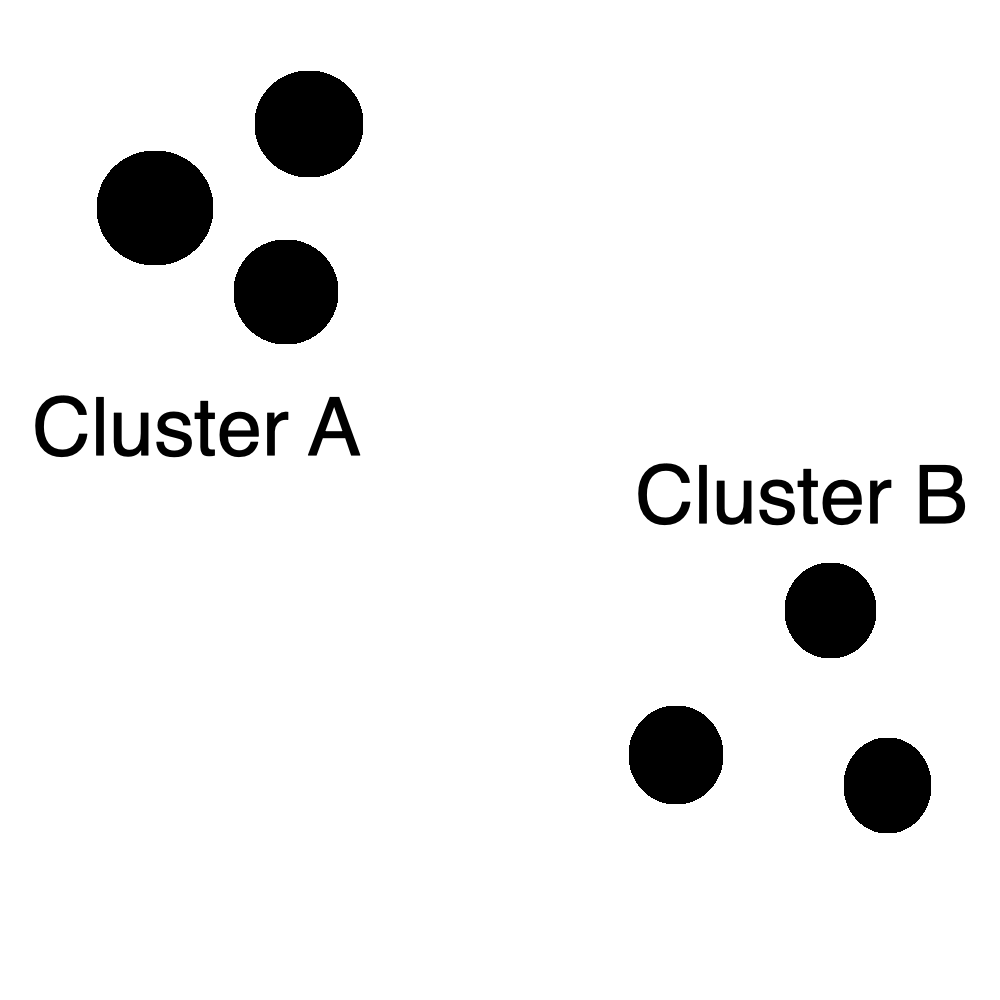
\includegraphics[width = 0.5\linewidth]{clusters_problem_6.png}
  \caption{Example of 2 clusters}
  \label{cluster}
\end{figure}


An example of heuristic to path this problem is to use create artificial data points that bridge the gap between the different clusters, resulting in the graph to become connected again. This could be achieved by using the fact that a disconnected neighbourhood graph implies that there exists clusters within the data and use the following scheme:

\begin{enumerate}
  \item Identify all $C_i, \; i = 1,2,...,k$ clusters by using the neighbourhood function G
  \item Pick a random point $p_i, \; i = 1,2,...,k$ of each cluster (the mean of the cluster would also work but harder to justify)
  \item Connect all points $p_i$ with each other using linspace$(p_i,p_j,n)$ where $n$ is chosen such that the distance between the artificial data points is equal to the smallest distance of the original data set.
\end{enumerate}

This would ensure that all clusters would be tied together as the distances between the artificial points equals the smallest distance of the original data set, ensuring that the artificial points will always belong to the neighbourhood sets of each other. The expected value of the distance between two clusters using this method will roughly correspond to the distance between the two cluster means. 
